\documentclass[fleqn,10pt]{wlscirep}
%\documentclass{article}
%\usepackage[margin=1in]{geometry}
\usepackage[utf8]{inputenc}
\usepackage[T1]{fontenc}
\usepackage{xspace}
\usepackage{url}
\usepackage{fancyvrb}
\usepackage{nameref}
\usepackage{hyperref}
\usepackage{graphicx}
\newcommand{\JournalTitle}[1]{#1}

\title{Application Level Cryptography for Securing Online Survey Responses}
\author{Simson L. Garfinkel and William Yates}
%\author[1,*]{Simson L. Garfinkel}
%\affil[1]{U.S. Census Bureau, Suitland, MD}
%\affil[*]{simson.l.garfinkel@census.gov}

%\keywords{Keyword1, Keyword2, Keyword3}

% Abstract goes here for Science abstract
\begin{abstract}
The second Privacy Impact Analysis of the EINSTEIN~3A system developed
by the U.S. Department of Homeland Security (DHS) indicated that the system would
have the ability to decrypt the TLS protocol used by the U.S. Census
Bureau to provide confidentiality for responses submitted using
internet self-response tools. To address this potential threat to
confidentiality, the Census Bureau designed an approach using the
World Wide Web Consortium's Web Cryptography API to provide a second
layer of cryptographic protection for respondent data. A working
prototype was developed. After further discussions with DHS, the
Census Bureau learned that the EINSTEIN~3A provisions for Web
Content Filtering were designed to decrypt outbound TLS connections
from U.S. Government facilities, and
not inbound connections from the general public to U.S. Government web
servers. However, the increased use of TLS decryption by other
organizations, the Census Bureau will continue to develop the
application level cryptography technology.
\end{abstract}


\newcommand{\ETA}{$\textrm{E}^\textrm{3}\textrm{A}$\xspace}

\begin{document}

%\flushbottom
\maketitle
% Abstract goes here for non-Science abstract
%\begin{abstract}
%\end{abstract}
%\thispagestyle{empty}

\section{Introduction}

The Census Bureau and other U.S. statistical agencies increasingly
rely on Internet-based self-response instruments to collect
data from individuals and establishments. Because Internet-connected
computers have long been under attack by both cyber criminals and
foreign governments~\cite{dick-testimony}, these connections are now
subject to monitoring by the U.S. Department of Homeland
Security (DHS).

Respondent data submitted to the Census Bureau website is protected
using the Transport Layer Security (TLS)~\cite{rfc8446} cryptographic
protocol and cannot be deciphered by DHS as the DHS monitoring system
is currently deployed.

Because the DHS system might change in the future in response to
new threats, the Census Bureau has developed and demonstrated an
approach that uses a second layer of encryption to protect respondent
data. This system would prevent DHS employees from accessing
respondent data even if DHS were to be provided with the Census
Bureau's TLS encryption keys.

\subsection{Background}

The Census Bureau and other U.S. statistical agencies collect
data from respondents under a pledge of confidentiality which states
that data collected will be used for statistical purposes
only. In particular, Title 13 of the U.S. Code prohibits information
that the Census Bureau collects from being used for law enforcement
purposes.

Statistical agencies are increasingly accepting data from respondents
using Internet self-response instruments. The Census
Bureau plans to make heavy use of Internet self-response for the 2020
census.~\cite{pennington2016} 
At the same time, computers operated by the U.S. Government are under
constant attack. A successful attack on Census Bureau computers would
also represent a significant threat to data confidentiality. For this
reason, the Census Bureau, like other civilian U.S. Government 
agencies, participates in the EINSTEIN network monitoring program
operated by the U.S. Department of Homeland Security.~\cite{thompson-feb2017}

At the 13th Biennial Federal Committee on Statistical Methodology
(FCSM) Policy Conference, a session explored ``The Challenges of
Overlapping Mandates between Federal Statistical Agencies and
Departmental Chief Information Officers.''~\cite{fcsm-program} One of
the panel speakers was Wayne R. Smith, the former Chief Statistician
of Canada and Head of Statistics Canada, who resigned his position in
September 2016 over concerns that the move to shared information services
meant that Statistics Canada would be unable to
protect the confidentiality of respondent
data~\cite{ottawacitizen}. After Dr. Smith spoke, several attendees
expressed concern that the U.S. Government's ``EINSTEIN'' program
might pose a similar threat to confidentiality for U.S. statistical agencies. 

\subsection{EINSTEIN}

The EINSTEIN program, operated by the U.S. Department of Homeland
Security (DHS), is designed to provide real-time collection,
analysis, and sharing of computer security information across the
federal civilian government to help mitigate threats.~\cite{dhs-einstein-2004}

The original EINSTEIN program was developed as part of the U.S.
Governments' Trusted Internet Connection program, an outgrowth of the
2003 National Strategy to Secure Cyberspace.~\cite{nstsc-2003}
The original EINSTEIN system was designed to
monitor and record network flow records between federal civilian executive branch
agencies and the public internet to provide after-action forensic analysis and support. The
EINSTEIN~2 program, first deployed in 2008, incorporated an intrusion
detection system to detect hostile activity against federal agencies
in real time and provide notification to the victims. Four years later, DHS began
transitioning to the EINSTEIN~3 Accelerated (\ETA) program, with the
goal of both detecting and preventing cyber attacks against federal
civilian government networks.~\cite{dhs-einstein}

Designed to be operated by the DHS Office of Cybersecurity and
Communications (CS\&C), EINSTEIN~3's feature set included deep packet
inspection, in which the content of network streams are examined by
the system. 

In April 2013, the Department of Homeland Security published 
\emph{Privacy Impact Assessment for EINSTEIN~3 --- Accelerated
  ($E^3A$)}~\cite{dhs-e3a-pia}. According to the PIA, ``\ETA combines
existing CS\&C analysis of EINSTEIN 1 and EINSTEIN~2 data as well as
information provided by cyber mission partners with existing
commercial intrusion prevention security services to allow for the
near real-time deep packet inspection of federal network traffic to
identify and react to known or suspected cyber threats.''~\cite[p.4]{dhs-e3a-pia}

The PIA explained that while deep-packet inspection might occasionally
result in the EINSTEIN~3 sensors encountering personally identifiable
information (PII), such information would be immediately deleted if it
was captured (see \nameref{excerpt1} on page~\pageref{excerpt1}). The PIA also stated that it
might be necessary, at times, to include PII captured by EINSTEIN in
an analytical product that DHS would then distribute. The PIA further
stated that non-cybersecurity information collected by DHS might be
disseminated for non-cybersecurity purposes (see \nameref{excerpt3} on
page~\pageref{excerpt3}).

On May 6, 2016, DHS issued an update to the \ETA PIA, stating that \ETA
would be enhanced with a new feature called Web Content
Filtering (WCF) that would provide the ability to decrypt
the Secure Socket Layer (SSL) protocol (see \nameref{excerpt4}). Note
that SSL
is the previous name for the TLS protocol that is
used to protect World Wide Web traffic.

Consistent with these stated capability improvements in the EINSTEIN
system, on December 14, 2016, the Census Bureau published a Notice in
the Federal Register indicating its intent to revise the
Census Bureau's confidentiality
pledge.~\cite{federal-register-2016-12-14} That new pledge has since
been adopted. It reads:

\begin{quote}
  ``The U.S. Census Bureau is required by law to protect your
  information. The Census Bureau is not permitted to publicly release
  your responses in a way that could identify you. Per the Federal
  Cybersecurity Enhancement Act of 2015, your data are protected from
  cybersecurity risks through screening of the systems that transmit
  your data.''~\cite{federal-register-2016-12-14,pledge}
\end{quote}

\subsection{Web Content Filtering of Encrypted Content}

Generally speaking, there are two ways that modern web browsers can
communicate with web servers over the Internet: by sending Hypertext
Transfer Protocol (HTTP) commands over the Internet without
encryption, and by wrapping HTTP commands within a TLS connection.

When a web page is accessed using a Uniform Resource Locator
(URL) that begins with ``http://'' --- for example,
\url{http://census.gov} --- the connection between the server and the
browser is not encrypted. Alternatively, when the same web page is
accessed using a URL that begins with ``https://''
(e.g. \url{https://census.gov}), then the server and the browser
exchange information over an encrypted connection.

By design, TLS
provides for both confidentiality and integrity of the connection: it
assures that a third party cannot eavesdrop on the contents of the
connection, and the data sent by the browser is received by the server
without modification.

TLS is based on public key cryptography. Each web server is configured
with a private key and a public key. Information encrypted with the
public key can only be decrypted using the corresponding private
key. The web server's public key and its hostname are stored in its
server certificate (Figure~\ref{tls}, step 1). When the web browser
connects to the web server (step 2), the server sends to the browser
the servers' certificate, which contains the public key (step 3). The
browser and the server then create a session key that is used to
encrypt the TLS connection (step 4).

\begin{figure}
  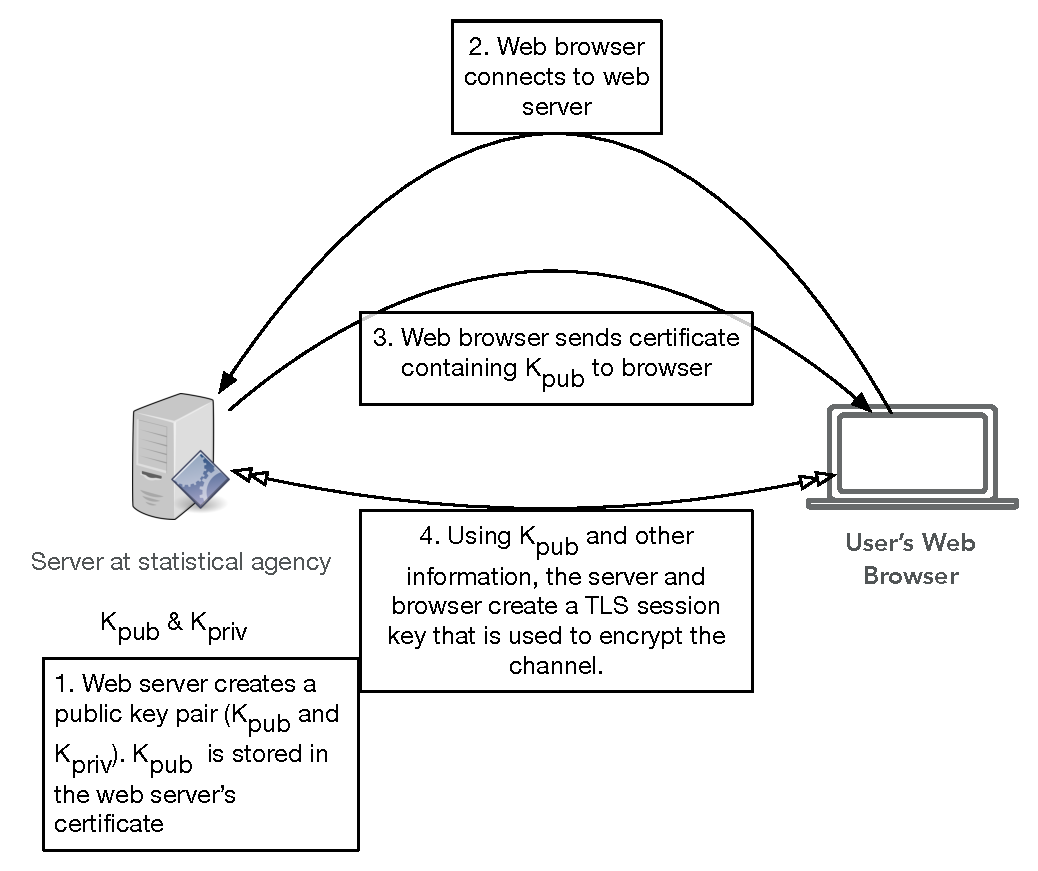
\includegraphics[width=\textwidth]{art/tls.pdf}
  \caption{The Transport Layer Security (TLS) protocol, in brief}\label{tls}
  \end{figure}

\begin{figure}
  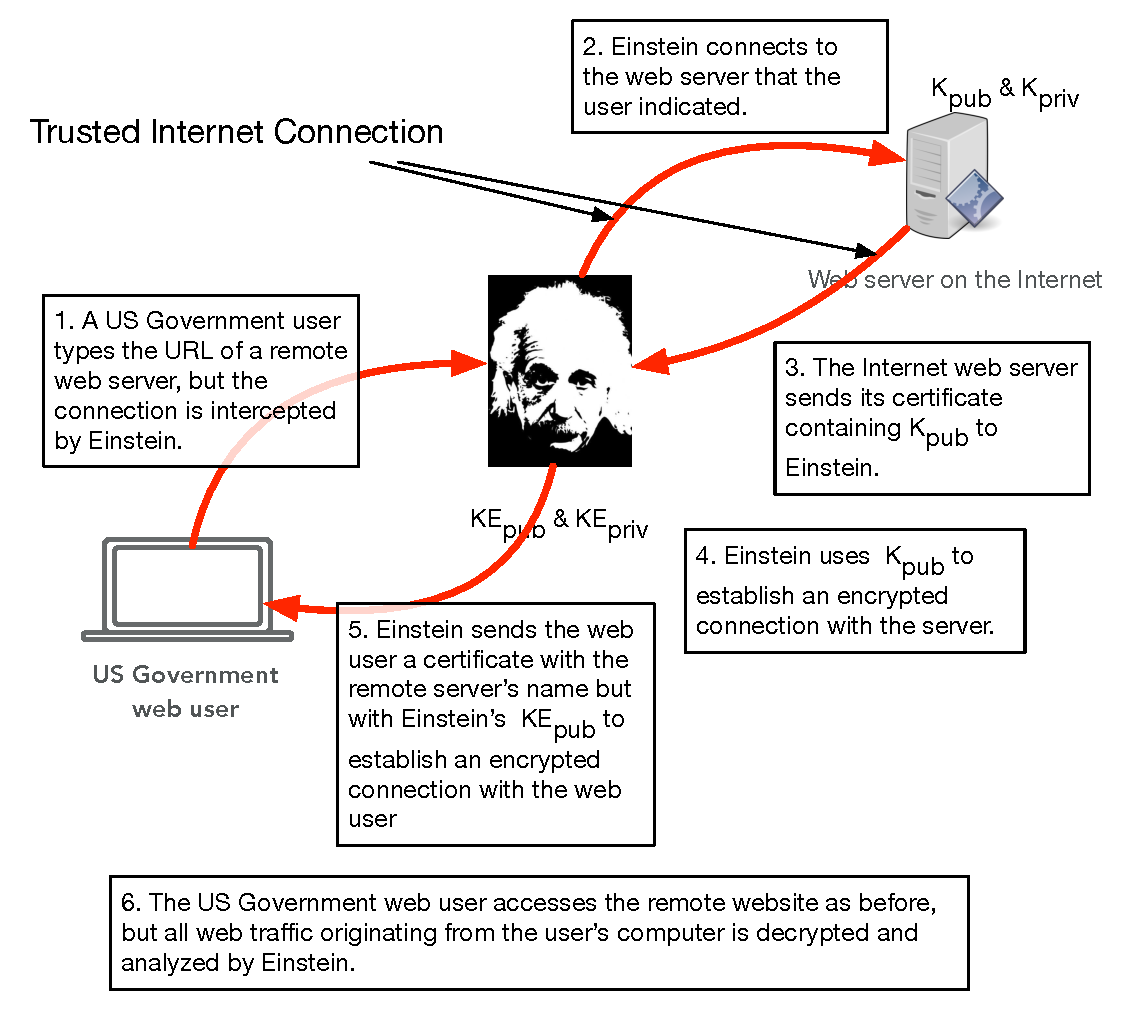
\includegraphics[width=\textwidth]{art/emonitoring1.pdf}
  \caption{EINSTEIN~3A's TLS interception capabilities as envisioned
    for monitoring outbound web connections of US Government employees.}\label{emonitoring1}
  \end{figure}

\begin{figure}
  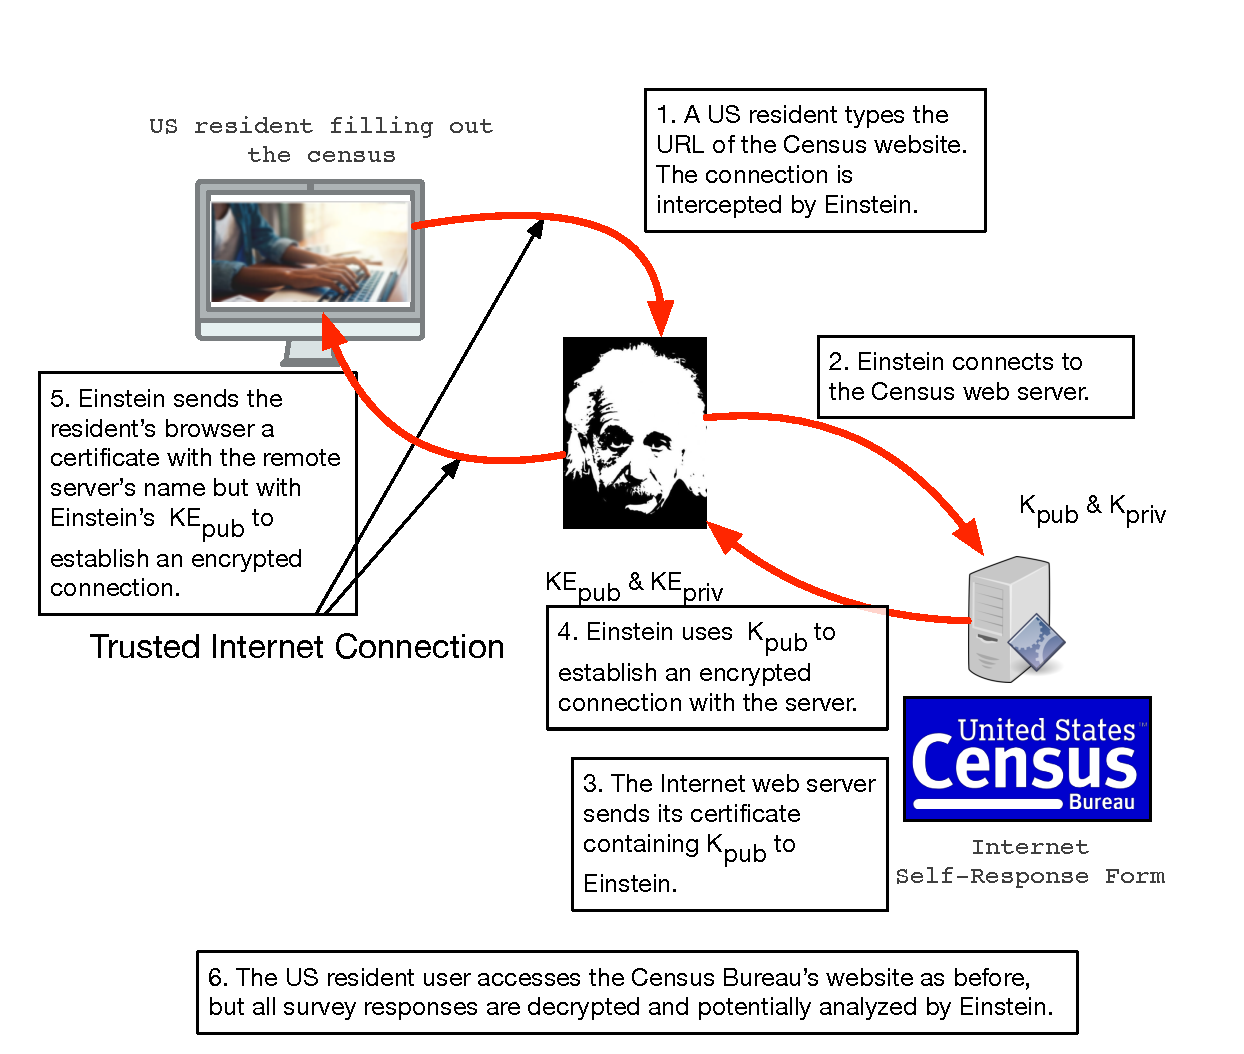
\includegraphics[width=\textwidth]{art/emonitoring2.pdf}
  \caption{EINSTEIN~3A's TLS interception could also be used to monitor the
    Census Bureau's Internet self response instrument.}\label{emonitoring2}
  \end{figure}

Many commercial network appliances now offer a feature variously
called ``Deep Packet Inspection of SSL/TLS Encrypted
Traffic''~\cite{sonicwall}, ``TLS Decryption,''~\cite{paloalto} and
``SSL analysis,''~\cite{globalsign}. These devices typically operate
as a cryptographic proxy, essentially mounting a relay attack on the
encrypted communications. TLS can't prevent this sort of attack, but
it allows the web browser to at least detect the attack, because the
certificate provided by the interception is not issued by a trusted
certificate authority.

The Web Content Filtering part of the DHS EINSTEIN~3A system
is designed to eavesdrop on the TLS-protected connection 
(Figure~\ref{emonitoring1}). When a web user at a U.S. Government
facility types  the URL of a remote web server (step 1), the browser opens a
connection not to the remote webserver, but to EINSTEIN~3A. It is the
EINSTEIN system that then makes the connection to the remote web
server (step 2). The remote web server sends its certificate back to
EINSTEIN (step 3), and the two systems create a cryptographically
protected channel that is used for future communication.
Finally, the EINSTEIN system sends its public key to the web user and
creates a second protected channel between EINSTEIN and the user (step
5). The browser's warning of an untrusted certificate can be overcome
by making the appliance a certificate authority and embedding the
appliance's certificate in the trusted certificate database of the web 
user's computer.

TLS interception systems similar to EINSTEIN are now widely used on the Internet.
A 2016 study by O'Neill et al. found that 1 in 250 TLS
connections on the Internet were proxied. ``The majority of these proxies appear to be benevolent,
however we identify over 1,000 cases where three malware
products are using this technology nefariously,'' the authors
concluded~\cite{DBLP:conf/imc/ONeillRSZ16}. There is also evidence
that foreign governments may have used this approach to spy on their
own citizens~\cite{fox-it-black-tulip}.

There are many reasons that an organization might legitimately wish to
monitor TLS connections in this manner. For example, the organization
could detect if a remote website was exploiting web browser
vulnerabilities to inject malware. TLS interception can also help
identify the command-and-control channels used by malware operating
within an organization, helping an organization to identify and
eliminate such electronic intrusions. Finally, TLS interception can be
used to detect inappropriate network activity by employees.

TLS interception systems can also be turned around, and used to
monitor inbound TLS connections to an organization's web server
originating on the public Internet
(Figure~\ref{emonitoring2}). In this configuration, the monitoring
system is given a copy web server's certificate and private key, so
that remote web users are not aware that they are connecting to the
monitoring device, rather than to the actual website. (TLS connections can be
monitored if the packets are captured and later decrypted using
the web server's private keys, although this approach does not work
for TLS version 1.3, which offers perfect forward secrecy.)

Given the widespread availability, use, and apparent acceptance of TLS
decryption technology, we sought to develop a system that would
protect respondent data even if the Census Bureau website was being
monitored with technology that decrypted TLS-protected communications. 
 
\subsection{Securing Respondent Data With the Web Cryptography API}

The World Wide Web Consortium's Web Cryptography API~\cite{wcapi}
defines a set of cryptographic functions that can be used by
JavaScript applications running in modern web browsers. According to the
standard, typical uses for this technology are to enable Multi-factor
Authentication, to encrypt documents locally that are then stored
encrypted on a remote website, to sign documents, and to implement
secure messaging. According to the Can I Use website, the Web
Cryptography API is well supported in all current web browsers except
for Internet Explorer 11 (Figure~\ref{caniuse}).

\begin{figure}
  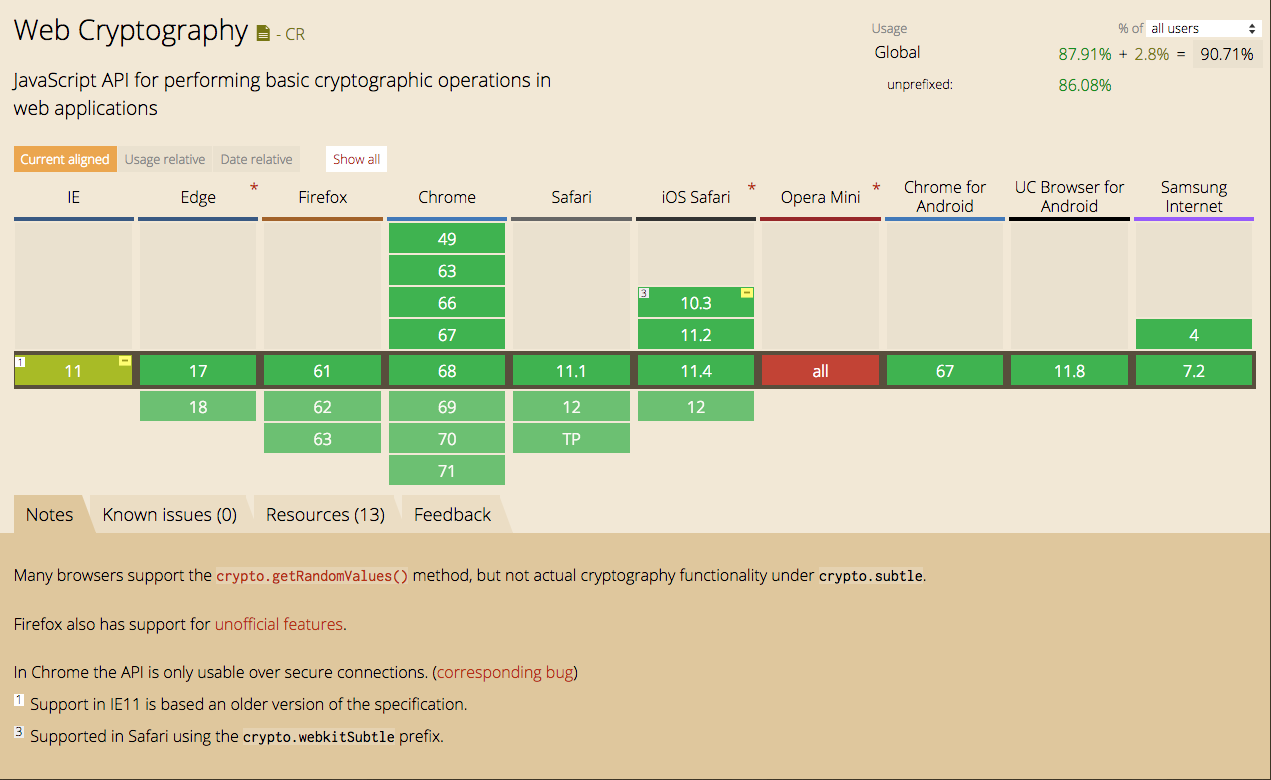
\includegraphics[width=\linewidth]{art/caniuse}
  \caption{Support for the Web Cryptography API as of September 2018,
    according to \url{https://caniuse.com/\#feat=cryptography}.\label{caniuse}}
\end{figure}

The Web Cryptography standard requires that web application using Web
Cryptography API be loaded into a web browser using the TLS protocol, in
order to assure that an attacker does not modify the JavaScript
application as it is being sent to the browser.

The Census Bureau has developed an approach that uses the Web
Cryptography API to encrypt survey responses sent from the
web browser to the web server separately from the underlying HTTPS
technology used to encrypt the web page itself (Figure~\ref{app-level-diagram}). This second layer of encryption
operates inside the HTTPS encrypted tunnel at the application data
level. The process beings with the web server at the statistical
agency creating a second encryption public key (Step 1) and used this second
key to encrypt respondent data, then sent the respondent data to the
web server for decryption. As a result, even if a TLS decryption
appliance was used to decrypt the HTTPS stream, it would not have
access to survey responses.

\begin{figure}
  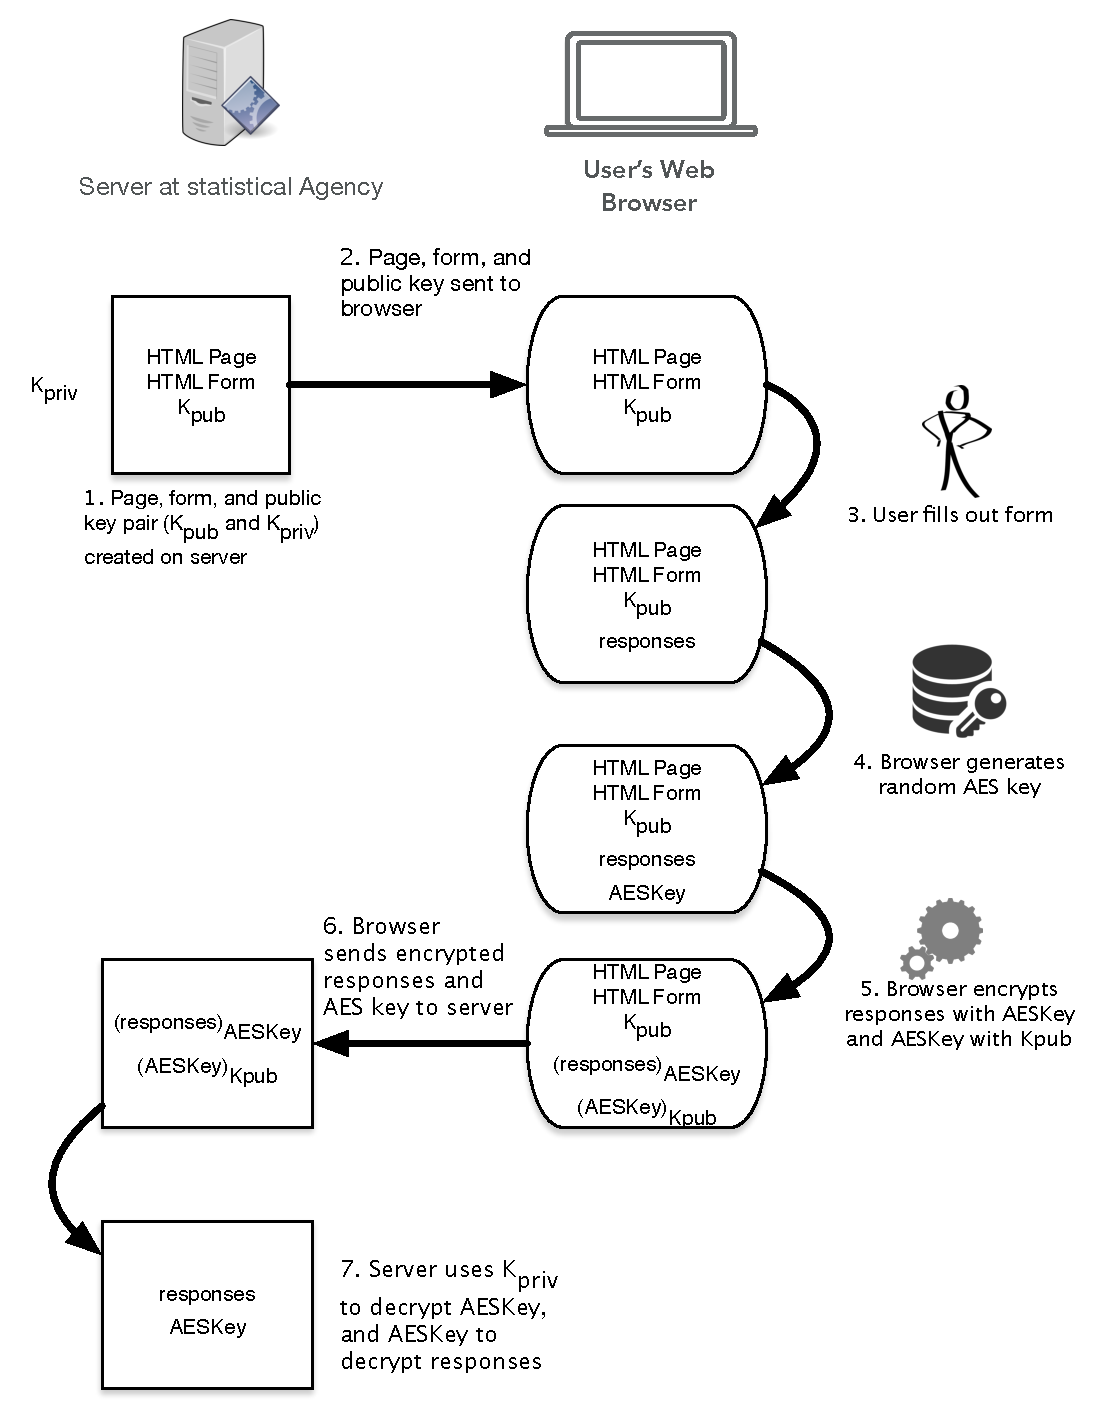
\includegraphics[width=\linewidth]{art/app-level-diagram}
  \caption{Application-level cryptography uses a second public/private
    key pair to encrypt survey responses.\label{app-level-diagram}}
\end{figure}

\subsection{DHS Reactions}

On October 13, 2017, a representative from the Census Bureau met with
representatives from the Department of Homeland Security's National
Cybersecurity Protection System (NCPS) to determine if the
application-level encryption system could be deployed without
violating any DHS policy and intentions~\cite{garfinkel-notes}. At the meeting, DHS
described the operation of the EINSTEIN system and the Census Bureau
described the application-level encryption approach. DHS stated that
deploying the application-level cryptography system would not violate
any DHS policy, and that the system
would provide additional security for Census Bureau-collected data, by
allowing the data to reside in encrypted form on the Bureau's web
server before it transited to a more secure system.

At the meeting, DHS also stated that in its current deployment, the \ETA Web Content Filtering
was not designed to filter data sent from external web browsers to
Government-operated web servers (e.g.~Figure~\ref{emonitoring2}). Instead, \ETA was solely designed to
monitor data sent between external websites and web browsers operated
within the government networks (e.g.~\Figure~\ref{emonitoring1}). For example, \ETA could intercept data
encrypted by malware running inside a user's web browser and
communicating with external web servers.

Following the October meeting, the Census Bureau arranged for DHS NCPS
to brief the Federal Committee on Statistical Methodology's
Confidentiality and Data Access subcommittee (which took place on
January 23, 2018), as well as the FCSM executive committee, to explain
that \ETA would not be deployed in a way that could decrypt respondent data.

\section{The Application Level Protection Mechanism}

This section describes the application level cryptography mechanism.

\subsection{Overview}

A typical Internet self-response survey consists of three parts:

\begin{enumerate}
  \item A web application server, which sends the survey form to
    the respondent, and receives the respondent data from the
    respondent's web browser.
  \item The survey form, which consists of a Hyper Text Markup
    Language (HTML) web page and associated JavaScript application
    that runs inside the respondent's web browser. The application
    presents the survey to the respondent, receives the data from the user, performs
    local data validation, and sends the data to the web application
    server.
  \item A database connected to the web application server, which stores responses.
\end{enumerate}

\subsection{Prototype}
In our development, we created two distinct prototypes.

The first prototype version encrypted each field of the survey form
using the plain RSA encryption using the PKCS1 v1.5
algorithm. This version of RSA encryption uses the OAEP-based
encryption scheme to protect against chosen plaintext and replay
attacks. The prototype is conceptually easy to understand, but it is not very efficient. 

Our second prototype used the generation of an AES-256 session
key to encrypt the JSON data structure, as described earlier in this
document. In this prototype, the RSA public/private keypair is
separately generated and the public key is explicitly embedded in the JavaScript; in a production
system, the public/private keypair would be stored in appropriately
protected files and dynamically served to the client. The keys are
created with the WebCryptography API and they are only valid for the
duration of the current page, per section 6.2 of the Web Crypto API standard.

Both prototypes implement a client/server system that displays a
simple survey, encrypts the survey results in the user's web browser,
and sends the encrypted results to the web server, where the encrypted
survey responses are stored in a database. A second interface, created
for a demonstration, shows both the encrypted and decrypted values.

Our prototype system modified the typical Internet survey system in the following ways:

\begin{enumerate}
\item The web application server was modified to create a second
  public/private key pair that is used to encrypt respondent
  data (Figure~\ref{app-level-diagram}, step 1).  We
  call this the application-level key pair. In our implementation, the
  server generates a 1024-bit RSA key pair that is used to secure all
  respondent data.
\item We modified the HTML and JavaScript application sent from web
  application server to the browser in three ways. First, the
  application-level public key is embedded in the JavaScript
  application. (step 2)
  
 The user fills out the HTML page as before (step 3).

\item We added additional JavaScript code that creates a 256-bit
  AES session encryption key to encrypt the respondent data when the user clicks the
  ``SUBMIT'' button (step 4). This session encryption key is then encrypted
  with the application-level public key (step 5).

   The encrypted session key and the encrypted respondent data (the ``encrypted
  package'') are sent to the  application server (step 6). 
\item We further modified the application server to store the encrypted
  package in the database.
\item Finally, we created a new program for extracting the encrypted
  data from the database and decrypting it. Decryption is performed
  using the application-level private key to decrypt the 256-bit AES
  session key, which is then used to decrypt the respondent data (step
  7).
\end{enumerate}


\subsection{Demo}

We create a simple web form for a hypothetical survey that requested a
first name and an age (Figure~\ref{survey}). When submitted, these two
values were packed into a JavaScript Object Notation (JSON) data
structure (Figure~\ref{json}), compressed, and encrypted with the session key. The
resulting data (Figure~\ref{encrypted}) was then sent to the web
server. We also created a user interface that demonstrated how the
data could be stored in the database either encrypted or decrypted (Figure~\ref{figure-demo}).

\begin{figure}
  \centering
  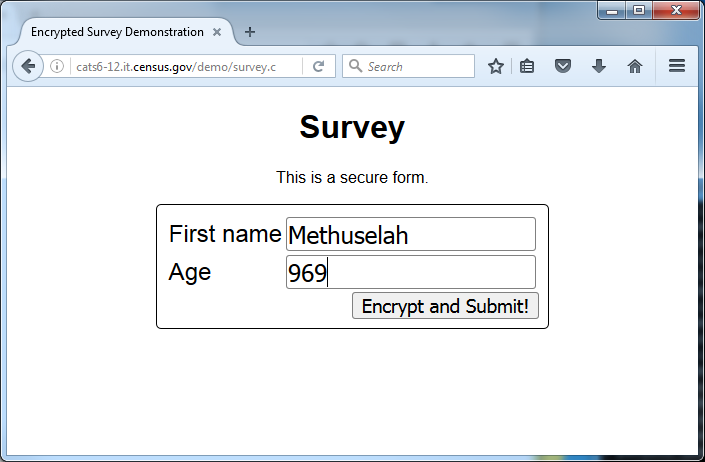
\includegraphics[width=.5\linewidth]{art/figure1}
  \caption{A hypothetical web survey instrument with sample data.}\label{survey}
  \end{figure}

\begin{figure}
  \begin{Verbatim}[frame=single]
    {"firstname":"Methuselah","age":"969"}
  \end{Verbatim}

  \caption{A JavaScript Object Notation (JSON) representation of the web response for Figure~\ref{survey}.}\label{json}
\end{figure}

\begin{figure}
  \begin{Verbatim}[frame=single]
    K4lCg6ZlNBi3Wj7jxGuCnPLBAtXVcCDb15yiPlc31bK0bIsXptQ/LC0kU1w4jdop
  \end{Verbatim}
  \caption{The contents of Figure~\ref{json}, compressed and encrypted.}\label{encrypted}
\end{figure}

\begin{figure}
  \centering
  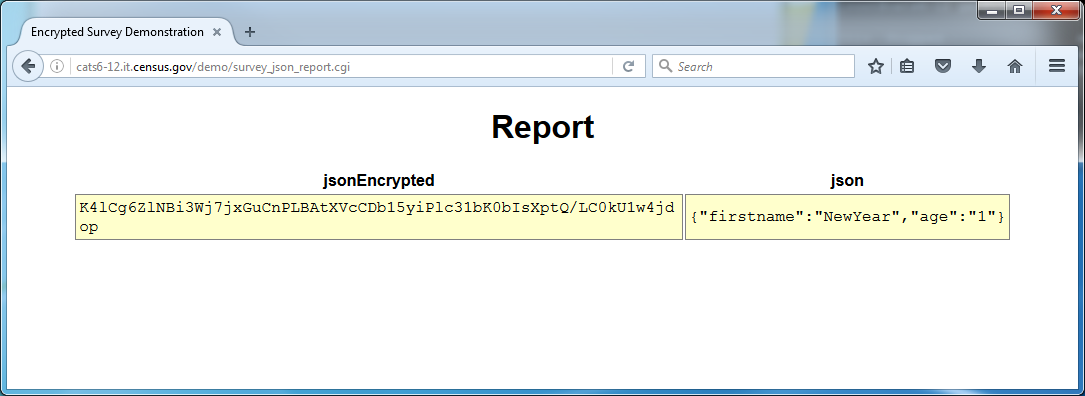
\includegraphics[width=.5\linewidth]{art/figure3}
  \caption{A user interface that was created for an internal
    demonstration that shows how either the encrypted JSON values or
    the JSON structure could be stored in a database.}\label{figure-demo}
  \end{figure}



\subsection{Source Code}
The prototype's source code is organized in two directories in the git repository:

\begin{description}
  \item[src/html/demo] Files for configuration and setup of the demo,
    as well as the JavaScript implementation.
  \item[src/cgi-bin/] Software that runs on the web server in response
    to the JavaScript running.
\end{description}

\subsubsection{src/html/demo}
This section describes the contents of the src/html/dmeo directory in
the git repository.

\begin{description}
  \item[config.ini] This configuration file specifies the location of
    the database, the database credentials, and a JSON object that
    specifies the public/private keypair. The key is specified with a
    JSON data object that specifies the parameters $d, e, q, n$ and $p$.
  \item[createdb.sql] The SQL schema for the server database.
  \item[dbutil.py] A python program that can create the database and
    list its contents.
  \item[demo\_random.html] A brief HTML demonstration of generating
    random numbers with JavaScript.
  \item[encrypt.js] JavaScript routines for using the Web Cryptography
    API, used for the first prototype.
  \item[encrypt\_json.js] A revised JavaScript encryption system that
    uses the \verb|window.crypto.subtle.generateKey()| function to
    create an AES-256 key, the \verb|JSON.stringify| method to marshal
    the form values, and the \verb|encrypt_buff| function to encrypt
    the JSON string.
  \item[jquery-3.1.1.min.js] The venerable JQuery JavaScript user
    interface library.
  \item[keyutil.py] A utility program or creating and manipulating
    the RSA keys used in the prototype.
  \item[keyutil\_test.py] Unit tests for the keyutil program.
  \item[notes.txt] Developer notes.
  \item[setup\_rel7.sh] A bash script that installs the necessary
    packages on a Red Hat Enterprise License (RHEL) System 7 Linux
    operating system to run the prototype.
  \item[survey\_json\_report.js] JavaScript for displaying the
      report of successfully encrypted and decrypted survey responses
      for the second prototype.
  \item[survey\_report.js] JavaScript for displaying the
      report of successfully encrypted and decrypted survey responses
      for the first prototype.
\end{description}

\subsection{/src/cgi-bin}
This section describes the contents of the src/cgi-bin directory in
the git repository. This directory contains the Common Gateway
Interface files that are used by the prototype; the files are stored
in a different directory because the RHEL7 secure configuration that
we used required that CGI scripts be stored in a different directory
than the HTML and JavaScript files.

\begin{description}

  \item[report.cgi] A CGI script that displays the secure form and
    shows the public key used to encrypt it.
    \item[submit.cgi] A CGI script that accepts the RSA-encrypted
      form, decrypts the parameters, and stores both the encrypted and
      decrypted values in the database. Note that this script was
      developed for demonstration purposes: in a production system,
      \emph{either} the encrypted or decrypted values would be stored
      in the database, depending on the deployment configuration.
      \item[submit\_json.cgi] A CGI submission script, used by the
        second prototype.
      \item[survey.cgi] A CGI script that displays the survey for the
        first prototype.
      \item[survey\_json.cgi] A CGI script that displays the survey
        for the second prototype.
      \item[survey\_json\_report.cgi] A CGI script that displays a
        report of the submitted values for the second prototype. 
      \item[survey\_report.cgi] A  CGI script that displays a
        report of the submitted values for the first prototype.
\end{description}        


\section{Conclusion}
We developed a system using the World Wide Web Consortium's Web
Cryptography API that would provide a second layer of cryptographic
protection for survey responses. This second layer was designed to
operate even if some kind of TLS decryption or Web Content Filtering
system was employed between the respondent and the internet
self-response instrument.

Although the system was
developed because of concerns over the Department of Homeland
Security's EINSTEIN~3A system, the Census Bureau learned during the
development of the system that EINSTEIN~3A was designed to monitor
\emph{outging} web traffic of U.S. Government employees, and not
\emph{incoming} traffic to U.S. Government websites.

Nevertheless, research by academics has determined that a small
percentage of Internet users have their web traffic monitored using
TLS interception techniques similar to those envisioned in the
EINSTEIN~3A program. An application-level encryption system would
protect respondents against this kind of monitoring. Application-level
encryption would also allow sensitive data to be collected by the
Census Bureau on Internet-connected servers and then to be transferred 
to internal servers at a later point in time for subsequent
decryption. As such, the Census Bureau will continue to work on this
technology, and hopes to produce a software toolkit that makes it easy
for web developers to use this approach at some point in the future.


\section{Disclaimer}
This paper is presented with the hope that its content may be of interest to the general statistical community. The views in these papers are those of the authors, and do not necessarily represent those of the Census Bureau.

%\bibliographystyle{plainurl}
\bibliography{app-level-crypto}

\section{Additional information}

\subsection{Excerpt from Privacy Impact Assessment for EINSTEIN~3---Accelerated (April 2013)}

\subsubsection{Relationship Between Participants --- Privacy Considerations}\label{excerpt1}
\begin{quote}
  ``CS\&C requires the ability to perform deep packet inspection of known or
suspected cyber threats that are identified by EINSTEIN sensors. CS\&C screens all data
captured by EINSTEIN 1 and EINSTEIN~2 sensors to ensure it is analytically relevant to
a known or suspected cyber threat. \ETA combines existing analysis of EINSTEIN 1 and
EINSTEIN~2 data as well as information provided by cyber mission partners with
existing commercial intrusion prevention security services to allow for the near real-time
deep packet inspection of federal network traffic to identify and react to known or
suspected cyber threats. Network flow records contain only packet header information.
Packet inspection tools allow an analyst to look at the content of the threat data, which
enables a more comprehensive analysis. Packet Capture may contain information that
could be considered PII-like malicious data from or associated with email messages or
attachments. CS\&C follows SOPs regarding handling of information that could be
considered PII including the deletion of any PII unless there is a connection to a known
or suspected cyber threat. Packet Capture shows details about the known or suspected
cyber threat within the federal network. CS\&C analyzes this detailed information and
issues warnings, including possible mitigation strategies to the threat.

  ``In accordance with the SOPs and information handling guidelines, all information
that could be considered PII is reviewed prior to inclusion in any analytical product or
other form of dissemination, and replaced with a generic label when possible. In some
cases, a product may include information that could be considered PII because that
information is deemed analytically relevant and necessary to understand the cyber threat.
In those instances, the SOPs and information handling guidelines provide for safeguards
regarding the marking, dissemination, and handling of the
information.''~\cite[p.9]{dhs-e3a-pia}
\end{quote}

\subsection{Privacy Impact Analysis: Related to Information Sharing}\label{excerpt3}
\begin{quote}
  \textbf{``Privacy Risk:} If non-cybersecurity information must be shared outside of DHS, it
increases the risk of unauthorized disclosure.

  \textbf{``Mitigation:} Information about known or suspected cyber threats collected,
analyzed, or otherwise obtained by CS\&C may be disclosed for cybersecurity purposes
and in furtherance of the DHS cybersecurity mission.

Information collected by \ETA or otherwise obtained by CS\&C may be
disseminated for non-cybersecurity purposes in limited situations when the collected
information appears to indicate involvement in activities that may violate laws or
otherwise when the sharing is done in the performance of a lawful government function.
This may include dissemination for law enforcement/intelligence or administrative
purposes unrelated to the protection of an information system from cybersecurity threats,
mitigations against such threats, or response to a cyber incident. In such cases, the
recipient will be a federal, state, or local law enforcement entity.''~\cite[p.23]{dhs-e3a-pia}
\end{quote}


\section{Excerpt from Privacy Impact Assessment Update for EINSTEIN~3---Accelerated (May 2013)}
\subsection{Reason for the PIA Update --- Web Content Filtering}\label{excerpt4}
\begin{quote}
``WCF will provide protection for web traffic5
by blocking
access to certain websites that are known to be, or include, malicious content (malware). In
addition, WCF will prevent malware from suspicious websites from running on federal civilian
Executive Branch D/A systems and networks. Finally, WCF will also detect and/or block phishing
attempts as well as the undesirable content that may be included in
those attempts.

``WCF categorizes web-based suspicious traffic, to include all URL/URIs and the content of web sessions,6 which allows system operators to specifically allow or disallow certain types of content that is known to be, or includes, malicious content (malware). WCF service can be configured to alert or block on traffic based on the applicable high-confidence cyber threat indicators and commercial signature development technology (used by the ISP) to allow DHS to block and alert against web-based traffic. This will permit traffic suspected by DHS as malicious as well as customer-specific cybersecurity risk protection requirements to alert or block on specific types of traffic. WCF provides this service via a web proxy between the client and the web server it is attempting to access. The proxy will perform the actions such as redirect, prevent, and/or alert on attempted access to certain (i.e., malicious) web content that matches a DHS cyber threat indicator that may look for a specific URL/URI or webpage content.

``WCF capabilities also include in-line Secure Socket Layer (SSL)
decryption; malware detection; and advanced analytics. WCF SSL
provides visibility into specific types of organizational traffic
(including web content) that has been encrypted, for the purpose of
protecting that traffic from malicious activity that would otherwise
remain hidden by traversing encrypted channels. The capability
decrypts web traffic of D/As participating in the \ETA WCF capability
for the purpose of detecting and preventing malicious web content on
the D/A network.  DHS is not interested in the behavior of
individuals; decryption is focused on web communications, not
communications between individuals. DHS does not use this capability
to investigate the behavior or private content of individuals. Malware
detection is an inherent part of operating WCF. WCF protects specific
federal civilian Executive Branch D/A traffic by using
Government-furnished cyber threat indicators to detect malicious
activity. Advanced analytics in this context refers to behavior-based
(heuristic) threat indicators to identify how a cyber threat or any of
the anomalous characteristics of a cyber threat, a computer system, or
the data behaves.''~\cite[pp 2--3]{dhs-e3a-pia2}.
\end{quote}

\end{document}

%% LocalWords:  cyber cryptographic cybersecurity mitigations NCPS TLS
%%  LocalWords:  FCSM decrypt decrypted cgi cryptographically
